\documentclass{standalone}
\usepackage{tikz}
\usepackage{ctex,siunitx}
\setCJKmainfont{Noto Serif CJK SC}
\usepackage{tkz-euclide}
\usepackage{amsmath}
\usetikzlibrary{patterns, calc}
\usetikzlibrary {decorations.pathmorphing, decorations.pathreplacing, decorations.shapes,}

\begin{document}
\small
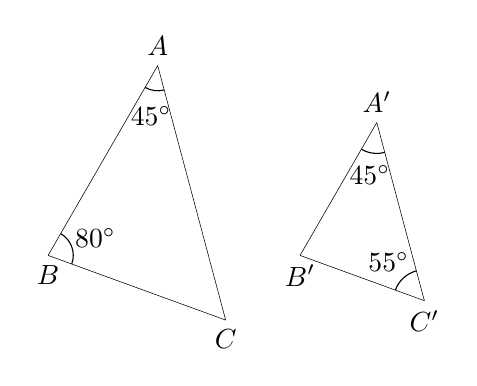
\begin{tikzpicture}[>=stealth,scale=0.8]
  \tkzSetUpPoint[fill=black]
  % \useasboundingbox(-1,-0.75)rectangle(3.7,1.4);
  \begin{scope}[rotate=-20]
  \tkzDefPoints{0/0/B, 3/0/C}
  \tkzDefPoint(80:3.48){A}
  \tkzDrawPolygon(A,B,C)
  \tkzMarkAngles[mark=none, size=.4](C,B,A B,A,C)
  \tkzLabelAngle[pos=.8](C,B,A){\ang{80}}
  \tkzLabelAngle[pos=.8](B,A,C){\ang{45}}
  \tkzLabelPoints[below](B,C)
  \tkzLabelPoints[above](A)
  \end{scope}
  \begin{scope}[xshift=4cm, scale=.7, rotate=-20]
    \tkzDefPoints{0/0/B', 3/0/C'}
  \tkzDefPoint(80:3.48){A'}
  \tkzDrawPolygon(A',B',C')
  \tkzMarkAngles[mark=none, size=.7](A',C',B' B',A',C')
  \tkzLabelAngle[pos=1.2](A',C',B'){\ang{55}}
  \tkzLabelAngle[pos=1.2](B',A',C'){\ang{45}}
  \tkzLabelPoints[below](B',C')
  \tkzLabelPoints[above](A')
  \end{scope}
\end{tikzpicture}
\end{document}